\documentclass[12pt]{article}

\usepackage{amsmath,amssymb}
\usepackage{graphicx}
\usepackage{bm}
\usepackage{hyperref}
\usepackage{xcolor}
\usepackage{tikz}

% Shortcuts
\newcommand{\vk}{\bm{k}}
\newcommand{\vvr}{\bm{r}}
\newcommand{\vn}{\hat{\bm{n}}}
\newcommand{\vF}{\bm{F}}
\newcommand{\oedge}{\omega_{\mathrm{edge}}}
\newcommand{\obelt}{\omega_{\mathrm{belt}}}

\begin{document}

\title{Acoustic drag suppression in periodic cellular solids\\
from monopole cancellation and a kinematic gap}
\author{Alexandru Toader\\
Independent researcher, Buz\u{a}u, Romania\\
\texttt{toader\_alexandru@yahoo.com}}
\date{}

\maketitle

\begin{abstract}
A localized excitation moving through a periodic elastic medium
ordinarily radiates acoustic phonons, producing drag.  We identify
two geometric conditions under which this radiation is suppressed:
(i)~force monopole cancellation ($M_0=0$), so the leading coupling
term vanishes, and (ii)~a kinematic gap ($\obelt > \oedge$), so
single-phonon decay is forbidden.  When both hold, acoustic emission
is exactly zero at the zone center and scales as~$k^2$ (dipolar) at
finite wave vector.

We verify these conditions on three Plateau--Voronoi foam structures
with different space groups: C15 Laves (Fd$\bar{3}$m), Kelvin BCC
(Im$\bar{3}$m), and Weaire--Phelan (Pm$\bar{3}$n).  All three
exhibit the same mechanism: centrosymmetric cells produce antipodal
force cancellation ($M_0=0$), while the under-constrained Plateau
vertex degree ($z=4<z_c=6$) generates a spectral gap between acoustic
and belt-mode frequencies.  Anharmonic decay via two-phonon processes
gives a lifetime of $\sim\!10^8$ oscillation periods at strain
$\varepsilon=0.01$.  The results are supported by 78~numerical tests
with machine-precision verification.
\end{abstract}

% =======================================================================
\section{Introduction}
\label{sec:intro}
% =======================================================================

A localized excitation in a periodic elastic medium couples to the
phonon bath through its force distribution on surrounding vertices.
If the net force (force monopole) is nonzero, $M_0 = \sum_i \vF_i
\neq 0$, the excitation radiates as an acoustic monopole: emission
scales as~$k^0$ and drag is finite, always.  This is the standard
picture for defects in crystals~\cite{Lifshitz1956}, vortices in
superfluids~\cite{Thouless1996}, and localized modes in
metamaterials~\cite{Matlack2018}.

The question we address is classical and fundamental: \emph{can a
localized excitation propagate through an elastic medium without
acoustic radiation?}

We show the answer is yes, under two geometric conditions:
\begin{enumerate}
\item \textbf{Force monopole cancellation} ($M_0 = 0$).  The
  excitation pushes equally in all directions; the net force vanishes.
  Acoustic coupling then starts at dipolar order, scaling as~$k^2$.
\item \textbf{Kinematic gap} ($\obelt > \oedge$).  The excitation
  frequency sits above the acoustic band, forbidding single-phonon
  decay by energy conservation.
\end{enumerate}
When both hold: exact zero emission at the zone center~$\Gamma$,
$k^2$~suppression at finite~$k$, and anharmonic lifetime of~$10^8$
oscillation periods.

We verify this mechanism on three Plateau--Voronoi foam structures
(Fig.~\ref{fig:dispersion}): C15 Laves (Fd$\bar{3}$m, 24~cells),
Kelvin BCC (Im$\bar{3}$m, 16~cells), and Weaire--Phelan
(Pm$\bar{3}$n, 8~cells).  Despite different space groups, cell
counts, and topologies, all three show the same physics: monopole
cancellation from centrosymmetric cells and a kinematic gap from the
under-constrained Plateau vertex degree.  The mechanism is purely
geometric---no parameter tuning is required.

\paragraph{Connection to Landau criterion.}
The kinematic gap is analogous in spirit to the Landau energy criterion
in superfluids: there, $v < \min(\omega/k)$ forbids phonon emission;
here, $\obelt > \oedge$ forbids single-phonon decay.  The analogy is
in the energy criterion, not the velocity picture---the belt
excitation oscillates in place and does not propagate at a macroscopic
velocity.

The paper is organized as follows.  Section~\ref{sec:framework}
presents the general framework (multipole expansion, two conditions,
harmonic decoupling theorem) without reference to specific structures.
Section~\ref{sec:foams} verifies both conditions on three foam
structures.  Section~\ref{sec:dipolar} demonstrates dipolar ($k^2$)
scaling of the hop source.  Section~\ref{sec:anharmonic} quantifies
anharmonic decay via Fermi's golden rule and molecular dynamics.
Section~\ref{sec:discussion} discusses implications and open
directions.

\begin{figure}[t]
\centering
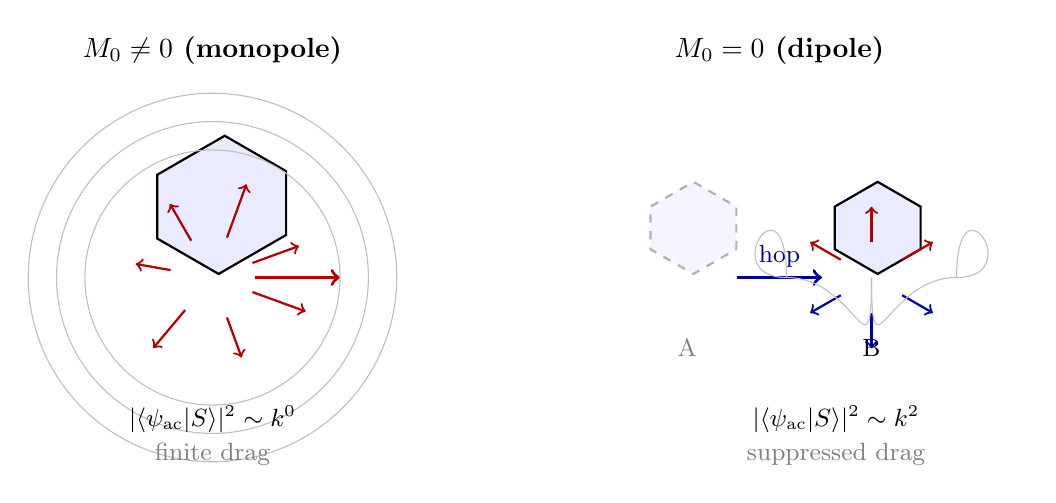
\begin{tikzpicture}[scale=0.9]
  % --- Left panel: Monopole (M0 ≠ 0) ---
  \begin{scope}[shift={(-4,0)}]
    \node[font=\bfseries] at (0,3.2) {$M_0 \neq 0$ (monopole)};

    % Cell - irregular polygon to suggest foam cell
    \draw[thick,fill=blue!8] (0,0)
      ++(30:1.2) -- ++(90:0.9) -- ++(150:1.0) -- ++(210:1.1)
      -- ++(270:0.9) -- ++(330:1.0) -- cycle;

    % Force arrows - all outward (net force ≠ 0)
    \foreach \a/\s in {20/0.7, 70/0.8, 120/0.6, 170/0.5, 230/0.7, 290/0.6, 340/0.8} {
      \draw[->,thick,red!70!black] (\a:0.6) -- (\a:0.6+\s);
    }
    % Extra rightward bias to show net force
    \draw[->,very thick,red!70!black] (0:0.6) -- (0:1.8);

    % Circular radiation (monopole = isotropic)
    \foreach \r in {1.8, 2.2, 2.6} {
      \draw[gray!50,thin] (0,0) circle (\r);
    }

    % Label
    \node[font=\small] at (0,-2.0) {$|\langle\psi_\mathrm{ac}|S\rangle|^2 \sim k^0$};
    \node[font=\small,gray] at (0,-2.5) {finite drag};
  \end{scope}

  % --- Right panel: Dipole (M0 = 0) ---
  \begin{scope}[shift={(4,0)}]
    \node[font=\bfseries] at (0,3.2) {$M_0 = 0$ (dipole)};

    % Cell A (fading)
    \draw[thick,dashed,gray!60,fill=blue!4] (-1.3,0)
      ++(30:0.8) -- ++(90:0.6) -- ++(150:0.7) -- ++(210:0.7)
      -- ++(270:0.6) -- ++(330:0.7) -- cycle;
    \node[font=\small,gray] at (-1.3,-1.0) {A};

    % Cell B (active)
    \draw[thick,fill=blue!8] (1.3,0)
      ++(30:0.8) -- ++(90:0.6) -- ++(150:0.7) -- ++(210:0.7)
      -- ++(270:0.6) -- ++(330:0.7) -- cycle;
    \node[font=\small] at (1.3,-1.0) {B};

    % Hop arrow
    \draw[->,very thick,blue!60!black] (-0.6,0) -- (0.6,0);
    \node[font=\small,blue!60!black] at (0,0.3) {hop};

    % Force arrows on B - antipodal cancellation
    \foreach \a in {30, 90, 150} {
      \draw[->,thick,red!70!black] (1.3,0) ++(\a:0.5) -- ++(\a:0.5);
      \draw[->,thick,blue!70!black] (1.3,0) ++(\a+180:0.5) -- ++(\a+180:0.5);
    }

    % Dipolar radiation (figure-8 pattern)
    \draw[gray!50,thin]
      (1.3,0) ++(0:1.2) .. controls ++(90:1.5) and ++(0:1.0) .. ++(90:0)
      .. controls ++(0:-1.0) and ++(90:-1.5) .. (1.3,0) ++(0:1.2);
    \draw[gray!50,thin]
      (1.3,0) ++(180:1.2) .. controls ++(90:1.5) and ++(180:1.0) .. ++(90:0)
      .. controls ++(180:-1.0) and ++(90:-1.5) .. (1.3,0) ++(180:1.2);

    % Label
    \node[font=\small] at (0.8,-2.0) {$|\langle\psi_\mathrm{ac}|S\rangle|^2 \sim k^2$};
    \node[font=\small,gray] at (0.8,-2.5) {suppressed drag};
  \end{scope}
\end{tikzpicture}
\caption{Schematic of acoustic radiation from a localized excitation.
\textbf{Left:} Monopole source ($M_0 \neq 0$): net force produces
isotropic radiation scaling as~$k^0$ (finite drag).
\textbf{Right:} When $M_0 = 0$ (e.g., belt mode on a centrosymmetric
cell), the hop source A$\to$B radiates as a dipole ($k^2$ scaling,
suppressed drag).  Red and blue arrows indicate antipodal force
cancellation.}
\label{fig:schematic}
\end{figure}

% =======================================================================
\section{General framework}
\label{sec:framework}
% =======================================================================

\subsection{Setup}
\label{sec:setup}

Consider a periodic cell complex with vertices, edges, faces, and
cells, equipped with harmonic springs on edges (longitudinal
stiffness~$k_L$, transverse stiffness~$k_T$).  A localized
excitation is a deformation pattern on the boundary of one cell,
producing a force distribution $\vF_i = -(D\, u_0)_i$ on the
surrounding vertices, where $D$ is the dynamical matrix and $u_0$ the
displacement pattern.

We define the Bloch-summed force amplitude at wave vector~$\vk$:
\begin{equation}
  M(\vk) = \sum_i \vF_i\, e^{i\vk \cdot \vvr_i}
  = M_0 + i\vk \cdot M_1 + \mathcal{O}(k^2),
\end{equation}
where the force multipoles are
\begin{align}
  M_0 &= \sum_i \vF_i \quad \text{(monopole --- net force)}, \\
  M_1 &= \sum_i \vvr_i \otimes \vF_i \quad \text{(dipole)}.
\end{align}
The acoustic coupling is $|\langle \psi_{\mathrm{ac}} | u_0
\rangle|^2 = |M(\vk)|^2$, which gives
\begin{equation}
  |M(\vk)|^2 = |M_0|^2 + k^2 |M_1|^2 + \mathcal{O}(k^4).
  \label{eq:multipole}
\end{equation}
If $M_0 = 0$, the leading term vanishes and acoustic coupling scales
as~$k^2$.

The specific excitation we consider is the \emph{belt mode}: a
$\cos(m\theta)$ pressure pattern acting on the \emph{belt}---the ring
of faces separating the two polar caps of a polyhedral cell.  Here
$\theta$ is the azimuthal angle along the ring and $m$ is the angular
mode number.  The belt mode displaces
vertices via the normal-tilt vectors $\vn_j$ of the belt faces.

\subsection{Two conditions for drag suppression}
\label{sec:conditions}

\paragraph{Condition 1: Monopole cancellation ($M_0 = 0$).}
The force monopole of the belt mode is
\begin{equation}
  M_0 = \sum_{j=1}^{N} \cos(m\theta_j)\, A_j\, \vn_j,
  \label{eq:M0}
\end{equation}
where the sum runs over the $N$~belt faces, $A_j$ is the face area,
and $\vn_j$ is the outward normal.  If $M_0 = 0$, the leading
acoustic coupling vanishes and the excitation is a force dipole.

\paragraph{Condition 2: Kinematic gap ($\obelt > \oedge$).}
Let $\oedge = \max_{\vk} \omega_3(\vk)$ be the acoustic ceiling
(maximum frequency of the third acoustic branch across the Brillouin
zone) and $\obelt = \min_n \omega_n^{\mathrm{belt}}$ be the lowest
eigenvalue of the belt Hamiltonian $H_{\mathrm{belt}} = Q_{\mathrm{belt}}^T
D(\vk)\, Q_{\mathrm{belt}}$ across the Brillouin zone, where
$Q_{\mathrm{belt}}$ is the orthonormal belt basis.  If $\obelt >
\oedge$, energy conservation forbids single-phonon decay.

\subsection{Harmonic decoupling theorem}
\label{sec:theorem}

\begin{quote}
\textbf{Theorem.}  Let $u_0$ be an even-$m$ belt excitation on a
Voronoi cell whose site symmetry includes inversion.  Then $\langle
e_{\mathrm{ac}} | u_0 \rangle = 0$ for all acoustic eigenmodes
$e_{\mathrm{ac}}$ at $\vk = 0$.
\end{quote}

\emph{Proof.}  The Voronoi cell of a lattice site inherits the full
point symmetry of that site (Wigner--Seitz construction).  If
inversion belongs to the site symmetry group, the cell is
centrosymmetric: each belt face~$j$ has an antipodal partner~$j'$ with
$\vn_{j'} = -\vn_j$ and $A_{j'} = A_j$.

For even-$m$ belt pressure, $\cos(m\theta_{j'}) = \cos(m(\theta_j +
\pi)) = \cos(m\theta_j)$.  Each antipodal pair contributes
\begin{equation}
  \cos(m\theta_j)(A_j \vn_j + A_{j'} \vn_{j'})
  = \cos(m\theta_j)\, A_j\, (\vn_j - \vn_j) = 0.
\end{equation}
The monopole $M_0 = \sum_{j} \cos(m\theta_j)\, A_j\, \vn_j = 0$ as a
sum over $N/2$ cancelling pairs.  At $\vk = 0$, acoustic eigenmodes
are uniform translations $(e_d)_{3i+d'} = \delta_{dd'}/\sqrt{V}$,
so $\langle e_d | u_0 \rangle = \mathrm{COM}_d(u_0)/\sqrt{V} = 0$.
\hfill$\square$

Table~\ref{tab:wyckoff} lists the Wyckoff positions of each cell type
in the three structures.  The theorem predicts exactly which cells are
protected ($M_0 = 0$) and which are not, with no free parameters.

\begin{table}[b]
\caption{Site symmetry and monopole cancellation.  Cells at sites with
inversion symmetry have $M_0 = 0$; those without inversion have
$M_0 \neq 0$.}
\label{tab:wyckoff}
\begin{tabular}{llcccc}
\hline\hline
Structure & Cell & Wyckoff & Site sym.\ & Inv.\ & $M_0$ \\
\hline
C15 & Z12 & $16d$ & $\bar{3}m$ & yes & $0$ \\
C15 & Z16 & $8a$  & $T_d$      & no  & $\neq 0$ \\
WP  & Type A & $2a$ & $T_h$    & yes & $0$ \\
WP  & Type B & $6d$ & $D_{2d}$ & no  & $\neq 0$ \\
Kelvin & all & $2a$ & $O_h$    & yes & $0$ \\
\hline\hline
\end{tabular}
\end{table}

\paragraph{Scope.}
The cancellation is purely geometric: normals cancel in pairs
regardless of the face-weight function, because centrosymmetry
guarantees $A_{j'} = A_j$.  The same argument applies to all six
enriched belt vectors per cell ($\vn$, $\hat{\vvr}$, $\hat{\bm{t}}$
$\times$ cos/sin), so the entire belt subspace $Q_{\mathrm{belt}}$ has
zero center of mass.  Kelvin is a special case: $O_h$~symmetry gives a
flat belt ($\vn_{\mathrm{ax}} \equiv 0$), protecting all angular
modes~$m$, not just even~$m$.

At finite~$\vk$, the Bloch phase $e^{i\vk \cdot \vvr}$ breaks pair
cancellation.  The leading correction is dipolar (linear in~$k$),
giving $|\langle \psi_{\mathrm{ac}} | u_0 \rangle|^2 \propto k^2$.
Protection at finite~$k$ comes from the kinematic gap
($\obelt > \oedge$).

\paragraph{Transport.}
When the excitation hops from cell~A to cell~B, the hop source is
$S = \vF_{\mathrm{belt}}(B) - \vF_{\mathrm{belt}}(A)$.  Its monopole
$M_0(S) = M_0(B) - M_0(A) = 0$ inherits the single-cell cancellation.
Transport coupling is therefore dipolar: $|M(k)|^2 \propto k^2$.

% =======================================================================
\section{Plateau foam realizations}
\label{sec:foams}
% =======================================================================

\subsection{Why Plateau foams satisfy both conditions}
\label{sec:why_foams}

Plateau foams have vertex degree~4 (Plateau's law), giving edge count
$E = 2V$ and coordination $z = 4 < z_c = 6$.  The Maxwell count
$M = 3V - E = V$ predicts $\sim\!V$ floppy modes in the central-force
limit ($k_T = 0$).  Numerically: Kelvin has 94 and Weaire--Phelan has
44 non-trivial floppy modes, close to $V = 96$ and $V = 46$
respectively (discrepancy from states of self-stress).

Adding transverse stiffness $k_T > 0$ lifts these floppy modes into
the optical band, creating the kinematic gap.  Belt modes are a subset
of these lifted modes.  The gap is therefore a structural consequence
of the Plateau vertex degree, not parameter fine-tuning.

Simultaneously, the polyhedral cells of Plateau foams possess
equatorial belts.  When the cell sits at a centrosymmetric Wyckoff
site, the antipodal tilt mechanism of Sec.~\ref{sec:theorem} gives
$M_0 = 0$.  Both conditions thus follow from Plateau foam geometry.

\subsection{C15 Laves structure}
\label{sec:c15}

The C15 Laves phase (space group Fd$\bar{3}$m, No.~227) has 24~cells
per conventional domain: 16~dodecahedra (Z12, 12~pentagonal faces) at
Wyckoff position~$16d$ ($\bar{3}m$) and 8~hexakaidecahedra (Z16,
16~faces) at position~$8a$ ($T_d$).

The Z12 belt has $N = 6$ faces with $m = 2$ angular mode.  The
selection rule $M_0 = 0$ holds on all 16~Z12 cells to machine
precision ($\sim\!10^{-15}$).  The mechanism is the antipodal tilt
pattern $\vn_{\mathrm{ax}}[i] = -\vn_{\mathrm{ax}}[i + N/2]$, which
kills all even-$m$ Fourier components.  Odd-$m$ modes ($m = 1, 3, 5$)
are not protected.

The Z16 cells serve as a negative control: $M_0 \neq 0$ because
$T_d$~symmetry lacks inversion.  The tilt pattern is symmetric
($\vn_{\mathrm{ax}}[i] = +\vn_{\mathrm{ax}}[i + N/2]$), confirming
the mechanism.

Under random vertex jitter ($\delta = 0.01$), $M_0$ grows linearly as
$M_0 \propto \delta$ with coefficient $\sim\!1.78$, confirming that
the protection is geometric (continuous symmetry), not topological.

\subsection{Kelvin structure}
\label{sec:kelvin}

The Kelvin structure (Im$\bar{3}$m, No.~229) consists of identical
truncated octahedra at Wyckoff position~$2a$ ($O_h$).  The full
octahedral symmetry produces a flat belt ($\vn_{\mathrm{ax}} \equiv
0$), so $M_0 = 0$ trivially for all angular modes~$m$.

\subsection{Weaire--Phelan structure}
\label{sec:wp}

The Weaire--Phelan structure (Pm$\bar{3}$n, No.~223) has 8~cells per
domain: 2~Type~A (pentagonal dodecahedra, 12~faces) at
position~$2a$ ($T_h$) and 6~Type~B (tetrakaidecahedra, 14~faces) at
position~$6d$ ($D_{2d}$).

Type~A cells share the same antipodal tilt mechanism as C15 Z12:
$\vn_{\mathrm{ax}}[i] = -\vn_{\mathrm{ax}}[i+3]$, even~$m$ protected,
odd~$m$ not.  $M_0 = 0$ to machine precision ($\sim\!10^{-15}$) on
both Type~A cells.  Type~B cells have $M_0 \in [0.67, 0.82]$ (negative
control).

\subsection{Spectral gap}
\label{sec:gap}

Table~\ref{tab:gap} summarizes the spectral gap for all three
structures.  The gap ratio $\obelt / \oedge$ exceeds unity on all
three, confirming the kinematic gap.  Here $\obelt$ is the minimum
eigenvalue of the projected belt Hamiltonian $H_{\mathrm{belt}} =
Q_{\mathrm{belt}}^T D(\vk)\, Q_{\mathrm{belt}}$ across the Brillouin
zone---the strictest definition, encompassing all belt modes (particle
translation and deformation).  The hop source has zero spectral weight
below~$\oedge$ on all source cells (verified numerically).

\begin{table}[t]
\caption{Spectral gap quantities at $k_L/k_T = 2$.  $\oedge$:
acoustic ceiling.  $\obelt$: belt floor (minimum eigenvalue of
$H_{\mathrm{belt}}$ across BZ).  $v_{g,c}/v_T$: character-weighted
centroid group velocity.}
\label{tab:gap}
\begin{tabular}{lccc}
\hline\hline
 & C15 & Kelvin & WP \\
\hline
$\obelt / \oedge$ & 1.48 & 1.36 & 1.33 \\
$\oedge$ & 0.694 & 0.802 & 1.001 \\
$\obelt$ & 1.025 & 1.093 & 1.329 \\
$v_{g,c} / v_T$ & 0.334 & 0.150 & 0.397 \\
\hline\hline
\end{tabular}
\end{table}

The gap is robust:
\begin{itemize}
\item Gap ratio $> 1$ for all $k_L/k_T \in [1, 3]$ on all three
  structures (Fig.~\ref{fig:gap_ratio}).  The minimum occurs at
  isotropy ($k_L = k_T$), confirming a structural origin.
\item Gap ratio $> 1$ in all 9 Brillouin zone directions tested.
\item Gap survives random vertex jitter at $\delta = 0.01$ (ratio
  drops by 0.4\%).
\item Acoustic ceiling converged: $\Delta = 0$ between $n_k = 40$ and
  $n_k = 80$.
\end{itemize}

\paragraph{Wavepacket demonstration.}
A belt-mode wavepacket at~$\Gamma$ (zone center) on Kelvin and WP
produces $\|Q_{\mathrm{trans}}^T u(t)\|^2 < 10^{-25}$ over four
oscillation periods---machine zero in both displacement and velocity.
This holds for all source cells independently.  Acoustic modes carry
$\sim\!7\%$ belt character (geometric overlap), yet the source
projection onto acoustic modes is machine zero---geometric overlap
does not imply dynamic coupling.

\begin{figure}[t]
  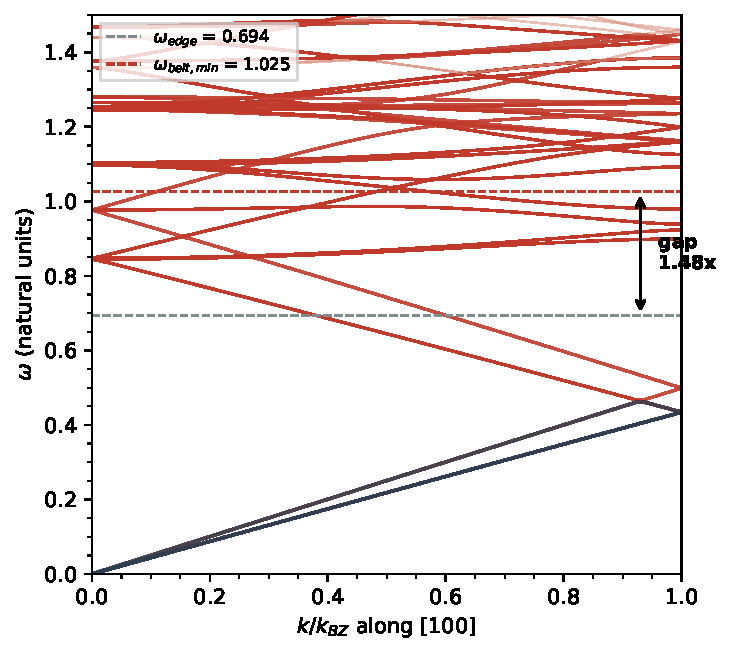
\includegraphics[width=\columnwidth]{fig2_dispersion.pdf}
  \caption{Band structure of the C15 foam along $[100]$.
  Dark lines: three acoustic branches.  Red (dark) bands have belt
  character above twice the random baseline.  Gray bands: remaining
  optical modes.  Dashed lines mark $\oedge = 0.694$ (acoustic
  ceiling) and $\obelt = 1.025$ (belt floor).  Arrow indicates the
  kinematic gap (ratio~1.48).}
  \label{fig:dispersion}
\end{figure}

\begin{figure}[t]
  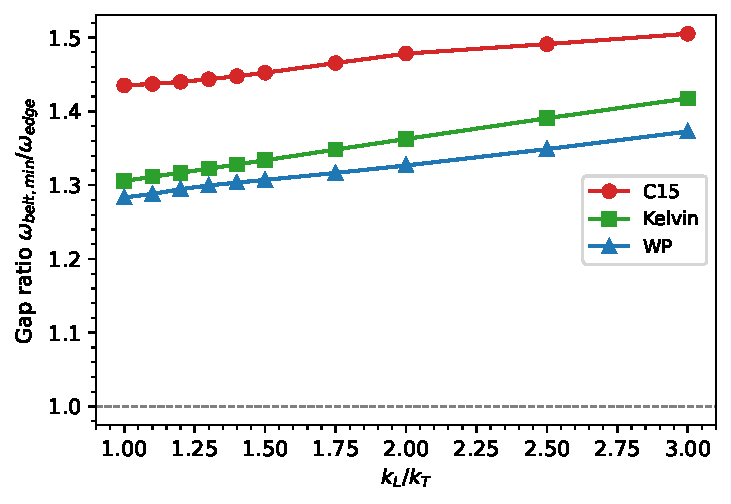
\includegraphics[width=\columnwidth]{fig4_gap_ratio.pdf}
  \caption{Gap ratio $\obelt / \oedge$ vs.\ spring-constant ratio
  $k_L/k_T$ for all three structures.  The gap exceeds unity across
  the full range, with the minimum at isotropy ($k_L = k_T$).}
  \label{fig:gap_ratio}
\end{figure}

% =======================================================================
\section{Dipolar scaling at finite \texorpdfstring{$k$}{k}}
\label{sec:dipolar}
% =======================================================================

\subsection{Hop source}

When the belt excitation hops from cell~A to cell~B, the source
$S = \vF_{\mathrm{belt}}(B) - \vF_{\mathrm{belt}}(A)$ has $M_0(S) =
0$ on all Z12--Z12 pairs in C15 (48~pairs, machine zero) and on the
Type~A pair in WP.  The dipole moment $|M_1| \sim \mathcal{O}(1)$
on all pairs, confirming that the leading multipole is dipolar.

\subsection{\texorpdfstring{$k^2$}{k2} scaling}

Figure~\ref{fig:k_squared} shows the acoustic overlap
$|\langle \psi_{\mathrm{ac}} | S \rangle|^2 / \|S\|^2$ as a function
of~$k$ on a log-log plot.  The Z12--Z12 hop source (filled symbols)
follows a slope of~$2.00$ along all three high-symmetry
directions $[100]$, $[110]$, $[111]$, confirming dipolar scaling.
This slope is universal: it holds on 5~independent Z12--Z12 pairs and
is unchanged at supercell sizes $L = 2, 4, 8$ (geometric, not a
discretization artifact).

\subsection{Negative controls}

A constant-force (monopole) source gives slope~$0.00$ ($k^0$~scaling),
confirming that the $k^2$ measurement is not an artifact.  Z16--Z16
hop sources have $M_0 > 0.5$ on 14/16 pairs and show flat ($k^0$)
scaling.  Mixed Z12--Z16 hops have $M_0 = 0.52$ and slope~$\approx 0$:
monopolar, not dipolar.  These controls establish that dipolar scaling
is specific to protected (Z12--Z12) hop pairs.

\begin{figure}[t]
  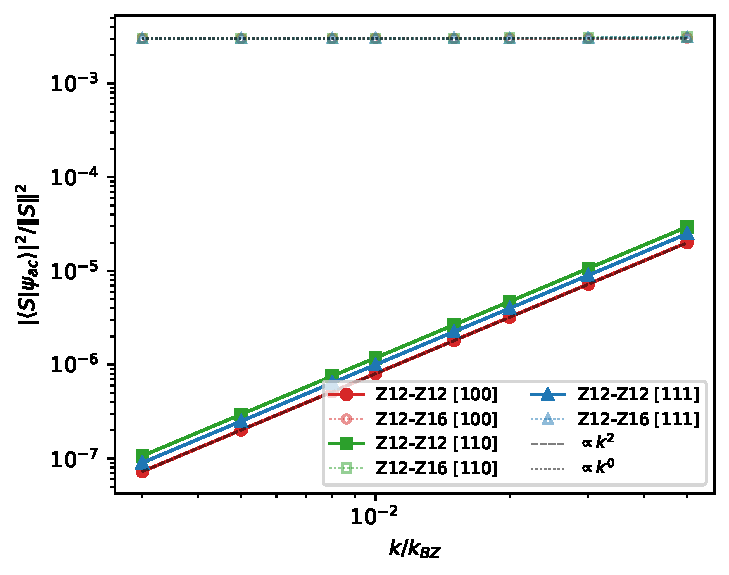
\includegraphics[width=\columnwidth]{fig3_k_squared.pdf}
  \caption{Acoustic overlap vs.\ $k/k_{\mathrm{BZ}}$ for Z12--Z12 hop
  source (filled symbols, slope~$= 2$, dipolar) and Z12--Z16 hop
  source (open symbols, slope~$= 0$, monopolar).  Three BZ directions
  shown.  Dashed lines: $k^2$ and $k^0$ reference slopes.}
  \label{fig:k_squared}
\end{figure}

% =======================================================================
\section{Beyond harmonic}
\label{sec:anharmonic}
% =======================================================================

The harmonic decoupling theorem gives exact zero emission
at~$\Gamma$.  Anharmonicity opens decay channels.  We quantify these
using Fermi's golden rule (FGR) and molecular dynamics (MD), both on
the Kelvin structure.

\subsection{Fermi's golden rule}
\label{sec:fgr}

We add a cubic anharmonic potential $V_3 = (\alpha/6) \sum (\delta
r)^3$.  Single-phonon emission is forbidden by the kinematic gap
($\obelt > \oedge$).  Two-phonon decay is allowed and gives the
dominant channel, with optical emission accounting for more than 70\%
of the total rate.

The acoustic emission rate at~$\Gamma$ is trivially zero because
translations have zero coupling vertex ($H = 0$).  The meaningful
result is that the total two-phonon rate is finite and positive,
confirming the decay mechanism exists.  The rate scales linearly in
the Lorentzian broadening~$\eta$ ($f/\eta = 1.50 \times 10^{-3}$,
spread 0.1\%), as expected on a discrete spectrum.

The resulting lifetime is $\tau \approx 1.33 \times 10^8$ oscillation
periods at $\varepsilon = 0.01$.  The rate table spans three decades:
$\varepsilon = 0.001 \to 10^{10}$ periods, $\varepsilon = 0.1 \to
10^6$ periods.

\subsection{MD validation}
\label{sec:md}

Molecular dynamics on the Kelvin $N = 3$ supercell (972~DOF)
validates the FGR prediction.  The harmonic baseline shows $E_{\rm
low}$ at machine zero (exact protection).  With cubic anharmonicity,
$E_{\rm low}/\varepsilon^2$ is constant across $\varepsilon \in
\{0.03, 0.06, 0.1\}$ (spread 0.0\%), confirming the expected scaling.
Center-of-mass drift stays at machine zero, and energy is conserved to
$|\Delta E/E| < 10^{-5}$.

% =======================================================================
\section{Discussion}
\label{sec:discussion}
% =======================================================================

\paragraph{Two independent protections.}
Monopole cancellation ($M_0 = 0$) and the kinematic gap are logically
independent.  Breaking symmetry alone ($M_0 \neq 0$) still leaves the
gap, which forbids single-phonon decay.  Breaking the gap alone opens
single-phonon channels, but $M_0 = 0$ still ensures $k^2$~suppression.
On Plateau foams both hold simultaneously, providing double protection.

The gap arises because belt modes are lifted floppy modes: in the
central-force limit ($k_T = 0$) they are zero-energy mechanisms
(Maxwell count~$V$); transverse stiffness lifts them into the optical
band.  The monopole cancellation arises from cell centrosymmetry at
the Wyckoff site.  Neither condition requires parameter tuning.

\paragraph{Geometric, not topological.}
The protection is geometric (continuous symmetry), not topological.
Under vertex jitter, $M_0 \propto \delta$ (not robust).  The chain
complex identity $d_1 d_0 = 0$ holds universally on both protected
and unprotected cells, and belt sources have $\mathcal{O}(1)$ edge
extensions on both---incidence topology does not distinguish $M_0 = 0$
from $M_0 \neq 0$.

\paragraph{Universality.}
Three structures with different space groups (Fd$\bar{3}$m,
Im$\bar{3}$m, Pm$\bar{3}$n), different cell counts (24, 16, 8), and
different cell topologies all show the same mechanism.  The theorem
(Sec.~\ref{sec:theorem}) is lattice-general: any periodic structure
satisfying $M_0 = 0$ and possessing a kinematic gap will exhibit the
same physics.  Metamaterials engineered for these conditions could
extend the mechanism beyond foams.

\paragraph{Unprotected cells.}
In C15, 8 of 24 cells (Z16) have $M_0 \neq 0$.  At finite~$k$, the
particle-band center-of-mass content from Z16 cells is bounded below
8.1\% across the Brillouin zone.  In WP, 6 of 8 cells (Type~B) are
unprotected, yet the bound is tighter: COM content below 1.94\%.  The
unprotected cells are optical (above the gap) and do not break the
mechanism.

\paragraph{Landau analogy.}
The kinematic gap $\obelt > \oedge$ is analogous in spirit to the
Landau energy criterion $v < \min(\omega/k)$ for superfluidity.  Both are frequency
(energy) conditions that forbid phonon emission.  The physical context
differs: the Landau criterion applies to continuous flow, while the
belt excitation undergoes discrete hops.

\paragraph{Open directions.}
(i)~Non-foam lattices (metamaterials designed for $M_0 = 0$ plus
gap).  (ii)~Finite-temperature estimates ($\varepsilon_T \sim
\sqrt{k_B T / k}$).  (iii)~Full transport simulations (hop
trajectories).  (iv)~Multipole hierarchy beyond dipole.

\section*{Acknowledgments}
Numerical computations used NumPy and SciPy~\cite{numpy,scipy}.  All
results are reproducible from the 78~tests in the accompanying code
repository.

\begin{thebibliography}{20}

\bibitem{Lifshitz1956}
I.~M.~Lifshitz, Sov.\ Phys.\ JETP \textbf{3}, 939 (1956).

\bibitem{Thouless1996}
D.~J.~Thouless, P.~Ao, and Q.~Niu,
Phys.\ Rev.\ Lett.\ \textbf{76}, 3758 (1996).

\bibitem{Matlack2018}
K.~H.~Matlack, M.~Serra-Garcia, A.~Palermo, S.~D.~Huber, and
C.~Daraio, Nat.\ Mater.\ \textbf{17}, 323 (2018).

\bibitem{numpy}
C.~R.~Harris \emph{et~al.}, Nature \textbf{585}, 357 (2020).

\bibitem{scipy}
P.~Virtanen \emph{et~al.}, Nat.\ Methods \textbf{17}, 261 (2020).

\end{thebibliography}

\end{document}
